%!TEX-program=pdflatexmk
%"runningheads" enables:
%  - page number on page 2 onwards
%  - title/authors on even/odd pages
%This is good for other readers to enable proper archiving among other papers and pointing to content.
%Even if the title page states the title, when printed and stored in a folder, when blindly opening the folder, one could hit not the title page, but an arbitrary page. Therefore, it is good to have title printed on the pages, too.
\documentclass[runningheads,a4paper]{llncs}

%Even though `american`, `english` and `USenglish` are synonyms for babel package (according to https://tex.stackexchange.com/questions/12775/babel-english-american-usenglish), the llncs document class is prepared to avoid the overriding of certain names (such as "Abstract." -> "Abstract" or "Fig." -> "Figure") when using `english`, but not when using the other 2.
\usepackage[english]{babel}

% See http://texdoc.net/texmf-dist/doc/latex/booktabs/booktabs.pdf and 
% chktex/chktex/chktexrc rules (!)
\usepackage{booktabs}

%better font, similar to the default springer font
%cfr-lm is preferred over lmodern. Reasoning at http://tex.stackexchange.com/a/247543/9075
\usepackage[%
rm={oldstyle=false,proportional=true},%
sf={oldstyle=false,proportional=true},%
tt={oldstyle=false,proportional=true,variable=true},%
qt=false%
]{cfr-lm}
%
%if more space is needed, exchange cfr-lm by mathptmx
%\usepackage{mathptmx}

\usepackage{graphicx}

%extended enumerate, such as \begin{compactenum}
\usepackage{paralist}
\usepackage{graphicx}
\usepackage{subcaption}

%put figures inside a text
%\usepackage{picins}
%use
%\piccaptioninside
%\piccaption{...}
%\parpic[r]{\includegraphics ...}
%Text...

%Sorts the citations in the brackets
%It also allows \cite{refa, refb}. Otherwise, the document does not compile.
%  Error message: "White space in argument"
\usepackage{cite}

\usepackage[T1]{fontenc}

%for demonstration purposes only
\usepackage[math]{blindtext}

%for easy quotations: \enquote{text}
\usepackage{csquotes}

%enable margin kerning
\usepackage{microtype}

%tweak \url{...}
\usepackage{url}
\urlstyle{same}
%improve wrapping of URLs - hint by http://tex.stackexchange.com/a/10419/9075
\makeatletter
\g@addto@macro{\UrlBreaks}{\UrlOrds}
\makeatother
%nicer // - solution by http://tex.stackexchange.com/a/98470/9075
%DO NOT ACTIVATE -> prevents line breaks
%\makeatletter
%\def\Url@twoslashes{\mathchar`\/\@ifnextchar/{\kern-.2em}{}}
%\g@addto@macro\UrlSpecials{\do\/{\Url@twoslashes}}
%\makeatother

%diagonal lines in a table - http://tex.stackexchange.com/questions/17745/diagonal-lines-in-table-cell
%slashbox is not available in texlive (due to licensing) and also gives bad results. This, we use diagbox
%\usepackage{diagbox}

%required for pdfcomment later
\usepackage[table,xcdraw]{xcolor}

% new packages BEFORE hyperref
% See also http://tex.stackexchange.com/questions/1863/which-packages-should-be-loaded-after-hyperref-instead-of-before

%enable hyperref without colors and without bookmarks
\usepackage[
%pdfauthor={},
%pdfsubject={},
%pdftitle={},
%pdfkeywords={},
bookmarks=false,
breaklinks=true,
colorlinks=true,
linkcolor=black,
citecolor=black,
urlcolor=black,
%pdfstartpage=19,
pdfpagelayout=SinglePage,
pdfstartview=Fit
]{hyperref}
%enables correct jumping to figures when referencing
\usepackage[all]{hypcap}

%enable nice comments
%\usepackage{pdfcomment}
%\newcommand{\commentontext}[2]{\colorbox{yellow!60}{#1}\pdfcomment[color={0.234 0.867 0.211},hoffset=-6pt,voffset=10pt,opacity=0.5]{#2}}
%\newcommand{\commentatside}[1]{\pdfcomment[color={0.045 0.278 0.643},icon=Note]{#1}}

%compatibality with TODO package
%\newcommand{\todo}[1]{\commentatside{#1}}
\usepackage{todonotes}

\usepackage{xspace}
%\newcommand{\eg}{e.\,g.\xspace}
%\newcommand{\ie}{i.\,e.\xspace}
\newcommand{\eg}{{\em e.\,g.,\/}}
\newcommand{\ie}{{\em i.\,e.,\/}}
\newcommand{\etc}{{\em etc.\/}}

\newcommand{\lfcomment}[1]{{\scriptsize\textcolor{red}{LF:~#1}}} 

%introduce \powerset - hint by http://matheplanet.com/matheplanet/nuke/html/viewtopic.php?topic=136492&post_id=997377
\DeclareFontFamily{U}{MnSymbolC}{}
\DeclareSymbolFont{MnSyC}{U}{MnSymbolC}{m}{n}
\DeclareFontShape{U}{MnSymbolC}{m}{n}{
    <-6>  MnSymbolC5
   <6-7>  MnSymbolC6
   <7-8>  MnSymbolC7
   <8-9>  MnSymbolC8
   <9-10> MnSymbolC9
  <10-12> MnSymbolC10
  <12->   MnSymbolC12%
}{}
\DeclareMathSymbol{\powerset}{\mathord}{MnSyC}{180}

% correct bad hyphenation here
\hyphenation{op-tical net-works semi-conduc-tor}

%%%%%%%%%%%%%%%%%%%%%%% CUSTOM %%%%%%%%%%%%%%%%%%%%%%%%%%%%%%%%%%%%%%%%%%%%%%%%
% Highlighting
\usepackage{soul}

% Glossaries and Acronyms
\usepackage[acronym]{glossaries} 
\newacronym{ast}{AST}{Abstract Syntax Tree}
\newacronym{ct}{CT}{Combinatorial Testing}
\newacronym{czt}{CZT}{Community Z Tools}
\newacronym{dap}{DAP}{Debug Adapter Protocol}
\newacronym{dbgp}{DBGP}{Common DeBugGer Protocol}
\newacronym{gui}{GUI}{Graphical User Interface}
\newacronym{ide}{IDE}{Integrated Development Environment}
\newacronym{lsp}{LSP}{Language Server Protocol}
\newacronym{poc}{PoC}{Proof of Concept}
\newacronym{pog}{POG}{Proof Obligation Generation}
\newacronym{po}{PO}{Proof Obligation}
\newacronym{slsp}{SLSP}{Specification Language Server Protocol}
\newacronym{vdm}{VDM}{Vienna Development Method}
\newacronym{vscode}{VS Code}{Visual Studio Code}
\newacronym{CSV}{CSV}{Comma Separated Values}
\newacronym{ISQ}{ISQ}{International System of Quantities}

% \makeglossaries   % Include to be able to print a glossary list
% \usepackage{acronym}
% \newacronym{ast}{AST}{Abstract Syntax Tree}
\newacronym{ct}{CT}{Combinatorial Testing}
\newacronym{czt}{CZT}{Community Z Tools}
\newacronym{dap}{DAP}{Debug Adapter Protocol}
\newacronym{dbgp}{DBGP}{Common DeBugGer Protocol}
\newacronym{gui}{GUI}{Graphical User Interface}
\newacronym{ide}{IDE}{Integrated Development Environment}
\newacronym{lsp}{LSP}{Language Server Protocol}
\newacronym{poc}{PoC}{Proof of Concept}
\newacronym{pog}{POG}{Proof Obligation Generation}
\newacronym{po}{PO}{Proof Obligation}
\newacronym{slsp}{SLSP}{Specification Language Server Protocol}
\newacronym{vdm}{VDM}{Vienna Development Method}
\newacronym{vscode}{VS Code}{Visual Studio Code}
\newacronym{CSV}{CSV}{Comma Separated Values}
\newacronym{ISQ}{ISQ}{International System of Quantities}

% \usepackage[color]{vdmlisting}
\usepackage{chngcntr}

%enable \cref{...} and \Cref{...} instead of \ref: Type of reference included in the link
\usepackage[capitalise,nameinlink]{cleveref}
%Nice formats for \cref
\crefname{section}{Sect.}{Sect.}
\Crefname{section}{Section}{Sections}
\crefname{lstlisting}{Listing}{Listing}
\Crefname{lstlisting}{Listing}{Listing}

% Code listings
\usepackage{listings} % Define the listing package
\usepackage{times}    % Prettier text in listings

% Code listing formatting for JSON
\lstdefinelanguage{json}{
    basicstyle=\ttfamily\small, 
    numbers=left,
    stepnumber=1,
    numbersep=8pt,
    breaklines=true,
    frame=single,
    xleftmargin=.11\textwidth, 
    xrightmargin=.11\textwidth
}

\usepackage{vdmlisting}

%%%%%%%%%%%%%%%%%%%%%%% Begin document %%%%%%%%%%%%%%%%%%%%%%%%%%%%%%%%%%%%%%%%
\begin{document}
% \counterwithout{lstlisting}{section}
%Works on MiKTeX only
%hint by http://goemonx.blogspot.de/2012/01/pdflatex-ligaturen-und-copynpaste.html
%also http://tex.stackexchange.com/questions/4397/make-ligatures-in-linux-libertine-copyable-and-searchable
%This allows a copy'n'paste of the text from the paper
%\input glyphtounicode.tex
\pdfgentounicode=1



%%%%%%%%%%%%%%%%%%%%%%%%%%%%%%%%%%%%%%%%%%%%%%%%%%%%%%%%%%%%%%%%%%%%%%%%%%%%%%%
\title{Topologically sorting VDM-SL definitions for Isabelle/HOL translation}
%TODO needs a better title!
%If Title is too long, use \titlerunning
%\titlerunning{Short Title}

%Multiple institutes are typeset as follows:
\author{Leo Freitas\inst{1} \and Nick Battle
}
%If there are too many authors, use \authorrunning
% \authorrunning{First Author et al.}
\authorrunning{ }

\institute{
%DIGIT, Aarhus University, Department of Engineering, \\
%Finlandsgade 22, 8200 Aarhus N, Denmark\\
%\email{\{jkr, fpm, hdm, pgl\}@ece.au.dk}
%\and
%Independent, \email{nick.battle@acm.org}
%\and
School of Computing, Newcastle University, \\
\email{leo.freitas@newcastle.ac.uk}
}
			
\maketitle
\setcounter{footnote}{0} 
\begin{abstract}
    There is an ecosystem of VDM libraries and extensions that includes a translation and proof environment for VDM in Isabelle~\footnote{\url{https://github.com/leouk/VDM_Toolkit/}}. Translation works for a large subset of VDM-SL and
    further constructs are being added on demand. A key impediment for novice users is the fact Isabelle/HOL requires 
    all definitions to be declared before they are used, where (mutually) recursive definitions \textbf{must} be defined in tandem. In this paper, we describe a solution to this problem, which will enable wider access to the translator plugin to novice users as well real models.   
\end{abstract}

\keywords{VSCode, VDM, Sorting}

%%%%%%%%%%%%%%%%%%%%%%%%%%%%%%%%%%%%%%%%%%%%%%%%%%%%%%%%%%%%%%%%%%%%%%%%%%%%%%%
\section{Introduction}\label{sec:intro}

The \gls{vdm} has has been widely used both in industrial contexts and academic ones covering several domains of the fields of Security~\cite{Kulik&20,Kulik&21a}, Fault-Tolerance~\cite{Nilsson&18}, Medical Devices~\cite{Macedo&08}, among others. We extend VDM specification support with a suite of tools and mathematical libraries~\footnote{\url{https://github.com/leouk/VDM_Toolkit/}}. 

VDM also has an \gls{vscode} IDE with multiple features, including a translation strategy to Isabelle/HOL~\cite{AdvancedVSCodePaper}. Nevertheless, the user needs to follow a strict and specific specification style. Otherwise, translation will either fail or be impossible. For example, every Isabelle/HOL theory \textbf{must} be written within a file of the same name, whereas VDM files might be moduleless or have multiple modules. Translation of such VDM modules will have to impose the required Isabelle style. Thus, users have to be aware of such issues, or else translation will fail.   

There are various such issues, which are listed in various example files in the distribution, and explained in detail in~\cite{NimFull}. These VDM ``idioms'' are important not only to enable translation, but also to ensure proofs will be manageable and proof strategies will be easier to identify. 

Nevertheless, a major impediment for use is the fact VDM specification \textbf{must} be ordered (\ie have declarations defined before they are used). This is rather unnatural to most VDM users, which tend to write specifications top-down, from larger/complex concepts to simpler/easier definitions. Also, it makes translation of legacy models hard because they were not written with such order requirement in mind. Manual rearrangement is not difficult, yet it is laborious and error prone, hence creating a barrier to entry for the translator. 

Solving this specific order requirement is the key contribution of this paper. We present the solution following the style by Naur's N-Queens algorithm~\cite{NQueens}:~we provide a historical account to how various developments within the VDM tools eventually led to the possibility of module sorting.  

%%%%%%%%%%%%%%%%%%%%%%%%%%%%%%%%%%%%%%%%%%%%%%%%%%
\section{Background}~\label{sec:background}

VDM translation is performed by traversing its abstract syntax tree (AST) and issuing corresponding Isabelle/HOL, for every part of the VDM concrete syntax that are compatible for translation. For example, VDM union types are quite expressive. They even allow some wacky definitions like this cross union selection example.
%
\begin{vdmsl}[frame=none,basicstyle=\ttfamily\scriptsize]
    types
        TUnion1 = int | nat
        inv u == (is_nat(u) => u > 0) and (is_int(u) => u < 0);

        TUnion2 = seq of nat | set of real;

    functions 
        f: TUnion2 * TUnion1 -> bool
        f(u2, u1) ==
            (is_int(u2) => 
                ((is_(u1, seq of nat) => u2 in set elems u1)
                  and
                 (is_(u1, set of real) => u2 in set u1))
            )
            and
            (is_nat(u2) => 
                ((is_(u1, seq of nat) => not u2 in set elems u1)
                  and
                 (is_(u1, set of real) => not u2 in set u1))
            );
\end{vdmsl}
%
VDM union types will create a maximal type set over the united types, where invariants are preserved. This can create quite complex (and confusing) selection and invariant checking processes. Of course, rarely such specifications are written. Yet, from a translation point of view, these are some of the challenges around VDM's expressivity with respect to how they can be translated to Isabelle. 

Another rather complex definition space in VDM are those for values and patterns. For example, one could define some pretty involved patterns in values and types like:
%
\begin{vdmsl}[frame=none,basicstyle=\ttfamily\scriptsize]
    types
        T = set of nat inv {a,b,c} == a < b and b < c;
    values 
        [i,j]: seq of nat = [1,2];
        {k,m}: set of nat = {2,1};
\end{vdmsl}
%
The type definition states it is an ordered set of explicitly three \verb'nat' values, whereas the values definitions bind each name to its corresponding value (\ie~\verb'i=1', \verb'j=2', where \verb'k' and \verb'm' will be a random choice within the set!). This poses various challenges for translation, given that Isabelle requires a stricter bindings between names, types and values. Practically, such examples are rerely an impediment (or rarely written), yet have to be handled by the sorting algorithm as well. In particular, value definitions like those of \verb'[i,j]' effectively create two separate value definitions for both \verb'i' and \verb'j'.   

That means the translator caters for the subset of VDM that is ``tamer'' (and mostly used). The translator has a VDM analysis tool (named \texttt{exu}\footnote{The name stems from the Yoruba divinity \textit{\`{E}\v{s}\`{u}} that was the gate keeper (and messenger) between mortals and deities.}), which checks for various such syntactic conondrums and limitations, telling users what to do and where problems are. Fixing such errors and warnings is important to ensure that translations are possible and without type errors for the user to solve on their own.  

\texttt{exu} also provides support to prepare users for translation (\eg~there are over \(50\) kinds of ``error'' and \(20\) ``warnings'' the translator can issue). For example, it checks that any function call within a function definition ought to include that function's precondition, if one exist. Yet, one key hindrance remained:~ordering of module definitions and their dependencies. This hindrance will be addressed in this paper and have recently been implemented in the latest versoin of the translator (see Section~\ref{sec:integration}). 

%%%%%%%%%%%%%%%%%%%%%%%%%%%%%%%%%%%%%%%%%%%%%%%%%%

\section{Important Historical Developments}\label{sec:history}

Before getting to our solution, it is important to identify key (unrelated) extensions to the main VDM tools. They were the stepping stones that eventually enabled \texttt{exu} to sort definitions for translation. We highlight the motivation for such extensions, as well as how they are implemented in the main VDM tools below.

\subsection{Load time problems}

When working with large VDM models~\cite{emv2} (\eg~\(150\)+ modules, \(60\)+ KLOC), typecheck time (\eg~\(2-4\) minutes) can become a hindrance, whereas initialisation time (\eg~\(15\)+ minutes) can compromise further development. 

Such long loading times occured because the VDM typechecker performs multiple passes through the AST in order to establishes whether all modules are 
consistent. The number of passes depends on the number of module inter dependencies (\ie~\texttt{module A} imports \texttt{module B} and vice-versa), order of declarations within modules (\ie~using definitions before defining them), \textit{etc.}. \lfcomment{Nick, any more here?}. 

Users of large models would have to keep track of dependencies by carefully checking import chains. For example, we had to carefully craft dependencies and keep their documentation explicitly. This was error prone and hard to maintain. 

\paragraph*{Verbose output.}
%
To address this, an extension was added to VDMJ that would track top-level type dependencies across modules. A simple and easy solution was for the typechecker to issue verbose output about every top-level definition dependencies as it traversed the VDM AST.\@ This required a tree visitor looking for dependencies and a mechanism for discovering free variables throughout the AST.\@ This verbose output enabled users to know how many passes have taken place, and whether cyclic dependencies existed and where. Users would then go and fix them manually. This meant one could use the verbose output to minimise passes by lowering dependencies, hence minimising load time.   

\paragraph*{Dependency and free variable visitors.}
%
In VDMJ~\cite{Battle09}, visitors are used to make specialised traversals over the AST.\@ For identifying module ordering, there are two visitors. The dependency visitor traverses the tree \lfcomment{Nick, explain here what the dependencies and free variable visitors do?}. 

\paragraph*{Topological sort of module dependencies.}
%
With the information gathered about dependencies, it was possible to create a topological sort of module names, where the result would be a list of module names with the fewest passes possible. This effectively solved (in most cases) the dependency warnings from the verbose output, hence giving the end user the ordered list of module names to load. This could then ge given to VDMJ at load time directly. This was enabled output of a acyclic directed graph view of module dependencies as a \texttt{dot} file.    

\subsection{Recursive cycles detection and removal.}

\lfcomment{Nick, maybe comment here the issues about mutual recursion and recursive type dependencies? And the tools / functionality they created?}

%%%%%%%%%%%%%%%%%%%%%%%%%%%%%%%%%%%%%%%%%%%%%%%%%%
\section{Exu ordering}\label{sec:exu}

Topological sort of dependencies worked inter modules and resolved the long load time issues. Nevertheless, it did not consider definitions within module themselves. Moreover, module dependency search did not consider local (\eg~\texttt{let-in} definitions) and funciton name spaces, where type name spaces were not checked. It was also related to top-level definition (\ie~types, values, functions, \etc) names rather than their structure.      

This required a different topological sort algorithm than the one available for module dependencies. The new algorithm consisted in five stages: 
%
\begin{enumerate} 
    \item Collect all named definitions
    \item Process non-function space dependenceies
        \begin{itemize}
            \item visit all definition dependencies 
            \item create any missing \verb'inv_T'
            \item link type with definition space  
        \end{itemize}
    \item Process function definition name-space dependencies 
        \begin{itemize}
            \item visit name-space dependencies 
            \item ignore recursive calls
            \item link named dependencies  
        \end{itemize}
    \item Topological sort
        \begin{itemize}
            \item Checks whether topological sorting is needed  
            \item Kahn's algorithm DAG sorting of top-level names 
         \end{itemize}
    \item Module reconstruction
         \begin{itemize}
             \item Organise top-level names to separate type from function name-spaces  
             \item Reorder module definitions 
             \item Optionally re-typechecks module 
          \end{itemize}
\end{enumerate}  
%
The first stage effectively flattens the module top-level definitions into a single list of everything being defined within the module. For example, explicit functions might define pre/postconditions as well as measures, whereas types might define invariant, equality or order predicates. Each of these definitions are explicit function themselves. 

The second stage seaches for top-level definition dependencies, where it creates invariant function definitions for all types that do not have them explicitly declared. This is important to ensure that every type \verb'T' without explicitly state invariants still depend on the function \verb'inv_T'. This effecitvely creates a function-space dependency between user-declared types, values and functions. Such synthetic constructs are structurally equivalent to what the typechecker would create had the user written something like \verb'inv_T = true' explicitly. This caters for the way both records and named typed invariant functions are constructed. For example, records create a function from the record name to boolean, whereas a named type \verb'S = RHS' creates a function from the \verb'RHS' type to boolean. Next, for declared values, there are no implicit functions to create, yet the named (type) dependency link is noted. This deeply process values, which can have multiple local definitions, as described in the examples above in Section~\ref{sec:background}.    

The third stage searches for free-variable dependencies across all top-level declarions, taking into account local contexts, such as function parameters or locally bound variables (\eg~quantified variables, let-def constructs, \etc). This search also finds recursive, as well as mutually recursive, function calls. The former are ignored/removed, given they are treated differently by the translator. The latter must be resolved, otherwise the topological search stage will fails, given it requires a directed acyclic graph (DAG). \lfcomment{Nick, could you add/say (or correct) here what other differences there are between TCDefinitionDependencies and TCFreeVariableVisitor?}    

The fourth stage is the actual topological sort algorithm used by VDMJ to sort module names described above. It is a variation of Kahn's DAG sort algorithm\footnote{\url{https://en.wikipedia.org/wiki/Topological_sorting\#Kahn's_algorithm}}. The DAG sort algorithm also looks for (and doe snot tolerate) cyclic dependencies within the given graph. Such cyclic dependencies have to be resolved earlier. In the case of definitions, cyclic dependencies can only occur between mutually recursive type of function definitions. Fortunately, VDMJ already has a mechanism for removing cyclic dependencies, which we apply here as well. This works well in practice. In the general case, however, this might fail, depending on the complexity of the mutual recursion(s) involved. \lfcomment{Nick, anything to add here?}

The first three stages are considered as the module definition processing phase. They create all the necessary structures and implicit definitions needed for sorting. Nevertheless, before the sorting itself, it is important to provide two sources of information. First, the sort has to be made based on so-called graph start points:~nodes without incoming links. Second, sorting is only to be attempted if the module does contain use of definitions before their declaration. That is because if you sort an already sorted module you can get an inconsistent result (\ie~a sorting order that does not prevent use before declaration). Thus, we ensure that Kahn's algorithm is only run when necessary. Whether it will be necessary is discovered based on a variation of VDMJ's verbose output warning for cyclic dependencis check. \lfcomment{Nick, anything else to say here regarding non-stability?}    

Finally, for the fitfh stage, if module sorting is not required, then the topological sorting is skipped and the module is not modified. Otherwise, if the sorting is requireed, then it is necessary to reorganise the topologically sorted list of names to take into account the two separate names spaces for types and functions at a module top-level definitions (prior to flattening definitions in the first stage). 

For example, consider the module \verb'M' below. It defines types and functions top-down, in use before declaration fashion, where some definitions do not have explicitly defined invariants. 
%
\begin{vdmsl}[frame=none,basicstyle=\ttfamily\scriptsize,numbers=left,stepnumber=1]
    module M 
    exports all
    definitions 
    types 
        --@doc uses types S and T before their declaration; implicit inv_Rec needed
        Rec:: s: S t:T;
        
        --@doc uses type T and function tail before declaring them.
        S = T inv s == head(s) > 0 and len tail(s) > 0;
        
        --@doc implicit inv_T needed
        T = seq1 of nat;

    functions
        tail: seq1 of nat -> seq of nat
        tail(s) == tl s;

        head: seq1 of nat -> nat
        head(s) == hd s;
    end M
\end{vdmsl}
%
If you run \verb'exu' (with the \verb'debug' flag set) on this module you get this output. 
%
\begin{vdmsl}[frame=none,basicstyle=\ttfamily\scriptsize]
    Calling Exu VDM analyser...
    Calculating declaration dependencies for module `M`...
    Printed dependencies for module M.dot at ./M.dot
    M`T declared after Rec
    M`S declared after Rec
    M`T declared after S
    tail declared after S
    tail declared after inv_S
    Found 5 definition use before declaration. Topological sorted required.
    Original names : Rec, S, T, tail, head
    Start points   : Rec, S
    Sorted names   : tail, head, inv_T, inv_S, T, inv_Rec, S, Rec
    Organised names: tail, head, T, S, Rec
    Exu successfully sorted module M definitions
\end{vdmsl}
%
The original names are the user defined top-level names in declaration order, which are available after the first stage. The start points are those names at the top of the graph (\ie~with no incoming links), which are available after the third stage as a sorted list of names by their declared location. The sorted names are the names after the fourth stage. Notice that it includes dependencies over (implicitily declared) type invariants for \verb'R' and \verb'T'. Finally, the organised names are those with both name-spaces consolidated containing only names within the originally declared set. 

Furthermore, notice that the order between functions \verb'head' and \verb'tail' and type \verb'T' is ``unstable'' (\ie~they are incomparable in this case). That is, whatever order they are declared is valid, so long as they are declared before \verb'S', which has to be declared before \verb'Rec'. It is these kinds of incomparibility between certain names that makes sorting modules where all names are declared before use can give irrelevant sorts. We try to minimise this by sorting the starting points by declaration order, but that cannot enterily prevent irrelevant sorts.  

The algorithm satisfies the invariant that the original and organised name sets are equal, and that the sorted names list contains all organised names. This way, all names are accounted and no implicitly created names (\eg~\verb'inv_T') are part of the result.     

Exu also produces a \texttt{dot} file view of the dependencies, which is similar to VDMJ's order plugin output for module name dependencies (see Figure~\ref{fig:Mdot}). It depicts the user declared dependencies before sorting. It includes corresponding source line locations, where starting nodes are tagged red with an inverted triangle shape, implicitly create invariants are double circles, and (terminal) nodes without outgoing links are shaped as a triangle.  
%
\begin{figure}[htbp]
    \centering
        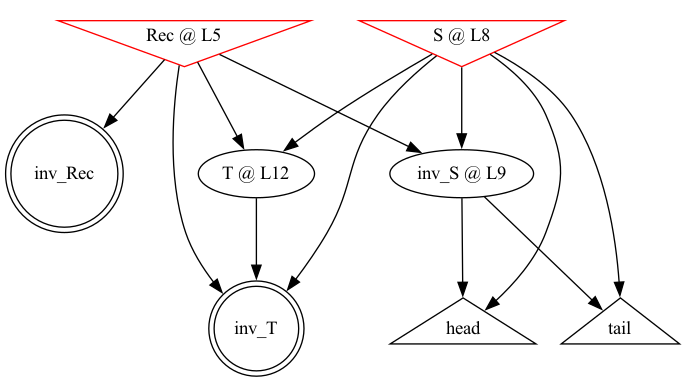
\includegraphics[width=\textwidth,scale=0.4]{figures/M.png}
    \caption{\texttt{M.vdmsl} definition dependencies.}\label{fig:Mdot}
 \end{figure}
%
For complex (and large) modules, such visualisation ``clues'' can be invaluable to figure out what tweaks to make in case unstable sorts produce results that are not entirely declaration before use and might generate Isabelle errors. 

%%%%%%%%%%%%%%%%%%%%%%%%%%%%%%%%%%%%%%%%%%%%%%%%%%
\section{VDMJ and VDM-VSCode integration}\label{sec:integration}

Our plugin infrastructure follows the Linux principle of strict separation between command line operations and their corresponding GUI outputs. The plugin architecture starts with a VDMJ \texttt{CommandPlugin} extension. This enables VDMJ console execution of the \texttt{exu} plugin via the command line. This plugin in setup, such that it will be used by all interfaces. 

For the VDMJ console interface, it follows the VDMJ convention that plugin classes are named according to the plugin call. The exposes functionality to the VDMJ debugging console like a call to a C/Java program \texttt{main} function with user-provided arguments.   

For the VDM-VSCode interface, it follows the LSP convetion that the plugin class incapsulates both GUI-editor reactive functionality as well as DAP command line debugging. For the DAP VDM debugging session, it offers the same VDMJ console plugin commands, where any issues or errors are reported to the DAP output console itself, as opposed to any GUI visualisations of such errors. This is mostly for debugging and low-level application purposes only. Users are encouraged to go via the GUI visualisation process instead. 

For the GUI visualisation process, the \texttt{ISA} LSP plugin reacts to two LSP events:~\textt{CompleteCheckEvent} and \texttt{UnknownTranslateEvent}. The former occurs after VDMJ has typechecked all loaded VDM-SL modules within a VDM-VSCode project, whereas the latter occurs when the user explicitly chooses the project pop-up menu for \verb'VDM->Translate to Isabelle'. 

For the \texttt{CompleteCheckEvent}, the plugin performs a staggered execution of aspects of the various plugins, including execution of \texttt{exu} for checking and sorting, \textit{vdm2isa} for translation, and \textit{isapog} for proof obligation translations. The result is the output of module definition dependency graphs, translation of both VDM source and proof obligations to Isabelle, as well as any errors and warnings that might have occurred during this process. 

For the \texttt{UnknonwnTranslateEvent}, VDM-VSCode-wide translation options are taken into account and the same process of processing modules for translation is performed. This is somawhat wasteful in the sense that translation happens both at right after typechecking time, and when the user explicit requests are made. This is a compromise on speed and usability:~if done  
For the \texttt{UnknonwnTranslateEvent}, VDM-VSCode-wide translation options are taken into account and the same process of processing modules for translation is performed. This is somawhat wasteful in the sense that translation happens both at right after typechecking time, and when the user explicit requests are made. This is a compromise on speed and usability:~the analysis for a successful translation is tightly couppled with what the translated output is supposed to be. Thankfully the ``lag'' time is reasonable on avrage and can be switcched off by the user (\ie~translation only occurs if the user asks via the \texttt{UnknownTranslateEvent} pop-up menu click). 

The trafe off for this use case is that errors are handled in tandem and only after a translation request has happened. If the \texttt{CheckCompleteEvent} processing is fast for the loaded project, then that is a preferred route for translation, as it will keep the user informed as the model is developed. Otherwise, translation can take place at the user's request and any remaining issues can be reported and dealt with accordingly.  

For the VDM-VSCode integration, we have strived to keep all three use cases (\ie~VDMJ console, VDM-VSCode DAP console, and VDM-VSCode LSP GUI-reactivity) as independent as possible, as well as reusable as possible. This is important so that each functionality does not need to be re-encoded in ever slightly different ways. This has been achieved through the use of he Linux principle of argument-based command-line execution of the plugin as a the bottom-line for all kinds of interfaces. 

In practice, this means each plugin responds to specific commands. This is similar to other Linux commands (\eg~)\texttt{git} has commands like \texttt{push}, \textt{pull}, \etc). Various default options are in place, and can be changed by a properties file. The property read and set process is close to VDMJ's own properties file. For VDM-VSCode, the GUI also exposes these properties through its settings interface. Ultimately, the VDM-VSCode plugin makes specific command calls to specific plugins, depending on whether it is part of the LSP's reactive behaviour  (\eg~setting yellow/red squiggles on code locations to show warnings/errors), or part of the DAP's interactive behaviour (\eg~calling specific DAP plugins on the debug console). Correspondingly, the same functionality is available through the VDMJ console via the command line. Output of translation is saved to \texttt{./.generated/isabelle} by default, yet users can set it to any directory of their choice. 

%%%%%%%%%%%%%%%%%%%%%%%%%%%%%%%%%%%%%%%%%%%%%%%%%%%%%%%%
\section{Applications and Examples}\label{sec:Examples}


Other examples of use are provided in the \texttt{ISQ.vdmsl} distribution~\footnote{\url{https://github.com/leouk/VDM_Toolkit/}}. They show various ISQ measurement systems in practical use.

%%%%%%%%%%%%%%%%%%%%%%%%%%%%%%%%%%%%%%%%%%%%%%%%%%%%%%%%
\section{Results and discussion}\label{sec:Results}

In this paper, we presented .

\paragraph*{Future work.}~
%
Future.

\paragraph*{Acknowledgements.}~
%
Acks.

%%%%%%%%%%%%%%%%%%%%%%%%%%%%%%%%%%%%%%%%%%%%%%%%%%%%%%%%%%%%%%%%%%%%%%%%%%%%%%%
\bibliographystyle{splncs03}
%\bibliography{refs.bib,au.bib,isq.bib}
\bibliography{order.bib}

% All links were last followed on November 13, 2022.
%%%%%%%%%%%%%%%%%%%%%%%%%%%%%%%%%%%%%%%%%%%%%%%%%%%%%%%%%%%%%%%%%%%%%%%%%%%%%%%

\end{document}
